\subsection{Les propriétés de BASE : }
Dans la première partie consacrée aux bases de données relationnelles nous avons vu les propriétés ACID auxquelles doivent répondre les SGBD de type relationnel. Les SGBD NoSQL qui, selon le théorème CAP, privilégient la disponibilité ainsi que la tolérance à la partition plutôt que la cohérence, répondent aux propriétés de BASE.

Le principe de BASE est le fruit d’une réflexion menée par Eric Brewer (Théorème de CAP). Les caractéristiques de BASE sont fondées sur les limites que montrent les SGBD relationnelles. Voici sa description :
\begin{itemize}[label=\textbullet]
\item \textbf{Basically Available :} quelle que soit la charge de la base de données (données/requêtes), le système garantie un taux de disponibilité de la donnée.
\item \textbf{Soft-state :} La base peut changer lors des mises à jour ou lors d'ajout/suppression de serveurs. La base NoSQL n'a pas à être cohérente à tout instant.
\item \textbf{Eventually consistent :} À terme, la base atteindra un état cohérent.
\end{itemize}

\begin{figure}[h]
	\centering
    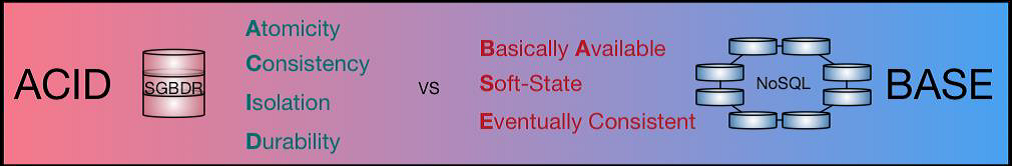
\includegraphics[scale=0.5]{img/part1/4.2}
    \caption{ACID vs BASE}
\end{figure}

Ainsi, une base NoSQL relâche certaines contraintes, telles que la synchronisation des réplicas, pour favoriser l'efficacité. Le parallèle ACID / BASE repris du domaine de la chimie permet d'appuyer là où ça fait mal : la concurrence. L'enfer des transactions gérées par les bases de données relationnelles est transformé en paradis pour le temps de réponse en relâchant cette contrainte impossible à maintenir.